\documentclass{article}
\usepackage{ulem}
\normalem
\usepackage{marvosym}
\usepackage{amssymb}
\usepackage{mathtools}
\usepackage{mathrsfs}
\usepackage{bm}
\usepackage{cite}
\usepackage{url,graphicx,tabularx,array,geometry}
%\usepackage{wasysym}
\usepackage{textcomp}
\usepackage{amsmath}
\usepackage{MnSymbol}
\usepackage{multicol}
\usepackage[affil-it]{authblk}
%\usepackage{mcode}
\usepackage{titling}
\newcommand{\subtitle}[1]{%
  \posttitle{%
    \par\end{center}
    \begin{center}\large#1\end{center}
    \vskip0.5em}%
}
\DeclareMathOperator{\Tr}{Tr}
\DeclareMathOperator{\rank}{rank}
\DeclareMathOperator{\Div}{div}
\DeclareMathOperator{\Log}{Log}
\DeclareMathOperator{\supp}{supp}
\DeclareMathOperator{\diag}{diag}
\DeclareMathOperator{\sign}{sign}
\DeclareMathOperator{\Alt}{Alt}
\DeclareMathOperator{\range}{range}

\topmargin=0.0in
\oddsidemargin=0.0in
\evensidemargin=0.0in
\textwidth=6.5in
\marginparwidth=0.5in
\headheight=0pt
\headsep=0pt
\textheight=9.0in

\newtheorem{theorem}{Theorem}
\newtheorem{defn}{Definition}
\newtheorem{lemma}{Lemma}
\newtheorem{cor}{Corollary}
\newtheorem{prop}{Proposition}

\title{Mathematics of Big Data I}
%\subtitle{d}
\author{Lecture 1: Overview of Big Data Analytics}
\date{September 5th, 2016}
\begin{document}

\maketitle

% 
%------------------------------------------------------------------------------
\section{Introduction -- The Big Picture of Big Data}

\noindent We will explore the key ideas of machine learning today to frame the subject.  We will answer

\begin{itemize}
\item Where does big data come from?
\item What are different ways of describing big data?
\item Data can be structured, semi-structured, or constructured.  How can we understand it?
\item What are the challenges with data (e.g. ``dirty" data)?
\end{itemize}

\noindent We will look at different methods of data processing, including ETL, data structuring, and dimensionality reduction.  Once we process data using these methods we will obtain a \textbf{data representation}.  These representations can include

\begin{itemize}
\item Discrete
\item Real-valued
\item Vector-valued
\item Matrix-valued
\item Manifold-valued
\item Mixed, etc.
\end{itemize}

\noindent We want to use data technology to get to ``data to decision" or D2D technologies.  All of these concepts fall under large subject called \textbf{machine learning}.  Within machine learning, we can \textbf{supervised} and \textbf{supervised learning}. 

\vspace{1pc}

\noindent The basics steps of D2D technologies include

\begin{itemize}
\item Data visualization
\item Mathematical modeling
\item Computational methods
\item Validation \& verification.
\end{itemize}

\noindent The key steps to doing this involves the same basic procedure:

\begin{enumerate}
\item Define a metric on your data space in order to define similarities (data points close in your metric space are ``similar").

\item Use strategies for effective optimization and computation  (we need to be able to discern which methods are faster and well-suited to the data we are processing).
\end{enumerate}

\noindent There are different \textbf{modeling approaches} we can take to new data.  These include \textbf{statistical calculus, geometric/analytic methods}, and \textbf{probability}.  Each one has it's own merit, but require different skill sets.  For instance, using the statistical calculus we could linear regression; geometric methods we will be able to see the answer intuitively; probabilistic methods are well-suited for machines since computers can quantify large amounts of data and many big data problems can be made into discrete probabilistic problems.  

\vspace{1pc}

\noindent Concepts we need to explore in all of this is to look at problems and see whether we can compute things globally or locally (like in the case of manifolds), and whether problems can be thought of either discretely or smoothly.  We can utilizing the power of computers using the following methods:

\begin{itemize}
\item Hadoop -- useful for large data sets
\item HDF -- useful for fault resilience
\item MapReduce -- useful for a ``divide and conquer" strategy
\item Spark -- useful for fast computation in memory, and
\item Zookeeper -- useful for orchestration.
\end{itemize}

\noindent Just as important as utilizing our computational tool set, we want to utilize mathematics to this end as well.  We will unify mathematics from

\begin{itemize}
\item Linear algebra
\item Statistics and Probability
\item Multivariable calculus
\item Geometry and discrete mathematics.
\end{itemize}

\noindent All of these concepts give us a big picture to all of the tools and concepts needed in data analytics.  In today's lecture we will explore the two questions of the origin of big data, and how we can represent it.  Later we will look at linear regression as an example of data analytics.

%%%%%%%%%%%%%%%%%%%%%%%%
\subsection{Where Does Big Data Come From?}

\noindent Big data comes from many sources.  Primarily we can get data from organizations such as retail stores.  Data also comes from machines.  For instance, an unmanned aerial vehicle (UAV), GPS devices, cell phones, computers, etc.  Lastly, people also generate data.  For instance, through social media, online shopping preferences, etc.  Data is not new, but in our modern era the scale of data has increased drastically.  The way people now use data is far different than it was in earlier generations.

%%%%%%%%%%%%%%%%%%%%%%%%
\subsection{What are the Types of Data?}

\noindent There are broadly speaking three types of data:

\begin{enumerate}
\item \textbf{Structured Data}: This type of data is often generated by organizations (for instance email data, shopping records).

\item \textbf{Semi-Structured Data}: This comes from machines typically.
\item \textbf{Unstructured Data}: This is often human-generated.
\end{enumerate}

%%%%%%%%%%%%%%%%%%%%%%%%
\subsection{What Exactly is ``Big" Data}

\noindent We might think that ``big" refers to volume, but it actually refers to five ``V"-words:

\begin{itemize}
\item Volume (size)
\item Velocity (speed)
\item Variety (types)
\item Veracity (quality)
\item Valence (relationships; multidimensional data often has dependencies on each other).
\end{itemize}

\noindent We can think of these 5 Vs as being the main points needed in order to master D2D technologies.  In Data to Decision we want to program machines to take actions based on data and learned knowledge.

% Analytic Approaches
%---------------------------------------------------------------------------------------
\section{Analytic Approaches -- Illustrating Big Data Analysis with Linear Regression}

\noindent There are three basic approaches to data analysis we discussed in the beginning:

%%%%%%%%%%%%%%%%
\subsection{Statistical Calculus Approach}

\noindent Our objective in data analysis is in reducing or minimizing the total error in our method.  However, the errors $e_i$ some could be positive and some could be negative.  We can't simply sum the errors since we run the risk of having zero error or negative error.  How can we fix this problem?  We can make error as something nonnegative.  We can consider an objective or cost function, for instance:

\begin{equation*}
J(m,b) \;\; =\;\; \sum_i e_i^2 \;\; =\;\; \sum_i (y_i - mx_i - b)^2.
\end{equation*}

\noindent This is an example of a quadratic.  Can we possibly use $\sum_i |e_i|$?  The answer is yes!  This is what's referred to as the $L^1$-norm, which can have many uses in data analysis.  

\vspace{1pc}

\noindent To illustrate this concept of a cost function, we will consider linear regression of sampled data points $(x_1, y_1), \ldots, (x_n, y_n)$.  The goal here is to find the line of best fit, or rather, find the best pairing $(m,b)$ for slope and $y$-intercept that minimizes the error in fitting these data points.  We can find the minimum of $J(m,b)$ with respect to these variables by finding the values of $m$ and $b$ where $\frac{\partial J}{\partial m} = 0$ and $\frac{\partial J}{\partial b} = 0$.  The partial derivatives here are given by 

\begin{eqnarray*}
\frac{\partial J}{\partial m} & = & \sum_i 2(y_i - mx_i - b)(-x_i) \\
\frac{\partial J}{\partial b} & = & \sum_i 2(y_i - mx_i - b)(-1).
\end{eqnarray*}

\noindent Since we are setting these both equal to zero, we can simply the coefficient $2$ in front of both of these equations.  To solve for $m$ and $b$ in these equations we have that 

\begin{eqnarray*}
m \sum_i x_i^2 + b\sum_i x_i & = & \sum_i x_iy_i \\
m \sum_i x_i + b\underbrace{\sum_i 1}_{=n} & = & \sum_i y_i.
\end{eqnarray*}

\noindent One method we can use is from linear algebra called {\em Cramer's rule}.  Essentially the method we are using above is by taking the gradient of the objective function $J$ and setting it equal to zero.  In general we can consider functions in the following situations:

\begin{enumerate}
\item \textbf{Single Variable}: These are the ordinary functions we see in single variable calculus which are $f:\mathbb{R} \to \mathbb{R}$.
\item \textbf{Many-to-One}: We can have scalar-valued functions of many variables $f:\mathbb{R}^n \to \mathbb{R}$.
\item \textbf{One-to-Many}: Functions of the form $f:\mathbb{R} \to \mathbb{R}^n$ define curves in higher-dimensional Euclidean spaces or manifolds.
\item \textbf{Many-to-Many}: Functions of the form $f:\mathbb{R}^n \to \mathbb{R}^m$ define $n$-dimensional vector fields embedded into $\mathbb{R}^m$.  Typically in this case we will use an upper case function of the form $\vec{F}:\mathbb{R}^n \to \mathbb{R}^m$ to denote vector fields.
\end{enumerate}

\noindent The way we take derivatives of each of these types of functions is different since we have to take derivatives with respect to different numbers of variables.  We will look at these more and more as time goes on.  

\vspace{1pc}

\noindent Returning to our example of linear regression, we would like to express our equations in a more compact form, by writing our equations in terms of a vector equation.  Instead of writing $J(m,b)$ in terms of a sum over it's components we can instead write

\begin{equation*}
\vec{y} \;\; =\;\; \left [ \begin{array}{c}
y_1\\
\vdots \\
y_n\\
\end{array} \right ] \hspace{3pc} \vec{x} \;\; =\;\; \left [ \begin{array}{c}
x_1\\
\vdots \\
x_n\\
\end{array} \right ]
\end{equation*}

\noindent and we can therefore write 

\begin{equation*}
J(m,b) \;\; =\;\; (\vec{y} - m\vec{x} -b) \cdot (\vec{y} - m \vec{x} - b)
\end{equation*}

\noindent where the $\cdot$ indicates the dot product.  We now want to take the gradient $\nabla J$ with respect to the variables $m$ and $b$.  Noting the product rule of functions $f,g:\mathbb{R}^n \to \mathbb{R}$ we obtain:

\begin{equation*}
\nabla (fg) \;\; =\;\; (\nabla f) g + f(\nabla g)
\end{equation*}

\noindent so therefore we compute

\begin{equation*}
0 \;\; =\;\; \nabla J \;\; =\;\; 2 \nabla(\vec{y} - m \vec{x} - b \textbf{1}) \cdot (\vec{y} - m\vec{x} - b\textbf{1})
\end{equation*}

\noindent and this implies the following equations:

\begin{eqnarray*}
(-\vec{x})\cdot (\vec{y} - m\vec{x} - b\textbf{1}) & = & 0 \\
(-\textbf{1}) \cdot (\vec{y} - m \vec{x} - b \textbf{1}) & = & 0.
\end{eqnarray*}

\noindent This can subsequently be written as 

\begin{eqnarray*}
\vec{x}^T\vec{y} - m \vec{x}^T\vec{x} - b\vec{x}^T \textbf{1} & = & 0 \\
\textbf{1}^T\vec{y} - m \textbf{1}^T\vec{x} - nb & = & 0 
\end{eqnarray*}

\noindent where we note that $\textbf{1}^T\textbf{1} = 1 + \ldots + 1 = n$ where we sum over all of the components of $\textbf{1}$.  There is in fact a more compact way of doing this.  If we instead make the substitutions $\vec{x}_0 = \textbf{1}$ and $\vec{x}_1 = \vec{x}$ we can instead write the compact equation

\begin{equation*}
\left [ \begin{array}{c}
\vec{x}_0^T \\
\vec{x}_1^T \\
\end{array} \right ] \left ( \vec{y} - \left [ \begin{array}{cc}
\vec{x}_0 & \vec{x}_1 \\
\end{array} \right ] \left [ \begin{array}{c}
b \\
m\\
\end{array} \right ] \right ) \;\; =\;\; 0.
\end{equation*}

\noindent Making the substitutions

\begin{equation*}
X \;\; =\;\; \left [ \begin{array}{cc}
\vec{x}_0 & \vec{x}_1 \\
\end{array} \right ] \hspace{3pc} \vec{\theta} \;\; =\;\; \left [ \begin{array}{c}
b \\
m \\
\end{array} \right ]
\end{equation*}

\noindent we find that 

\begin{equation*}
X^T(\vec{y} - X \vec{\theta}) \;\; =\;\; 0
\end{equation*}

\noindent  and therefore $X^TX \vec{\theta} = X^T\vec{y}$.  In the case that $X^TX$ is invertible we can solve this explicitly as $\vec{\theta} = (X^TX)^{-1}X^T\vec{y}$.  

\vspace{1pc} 
\centerline{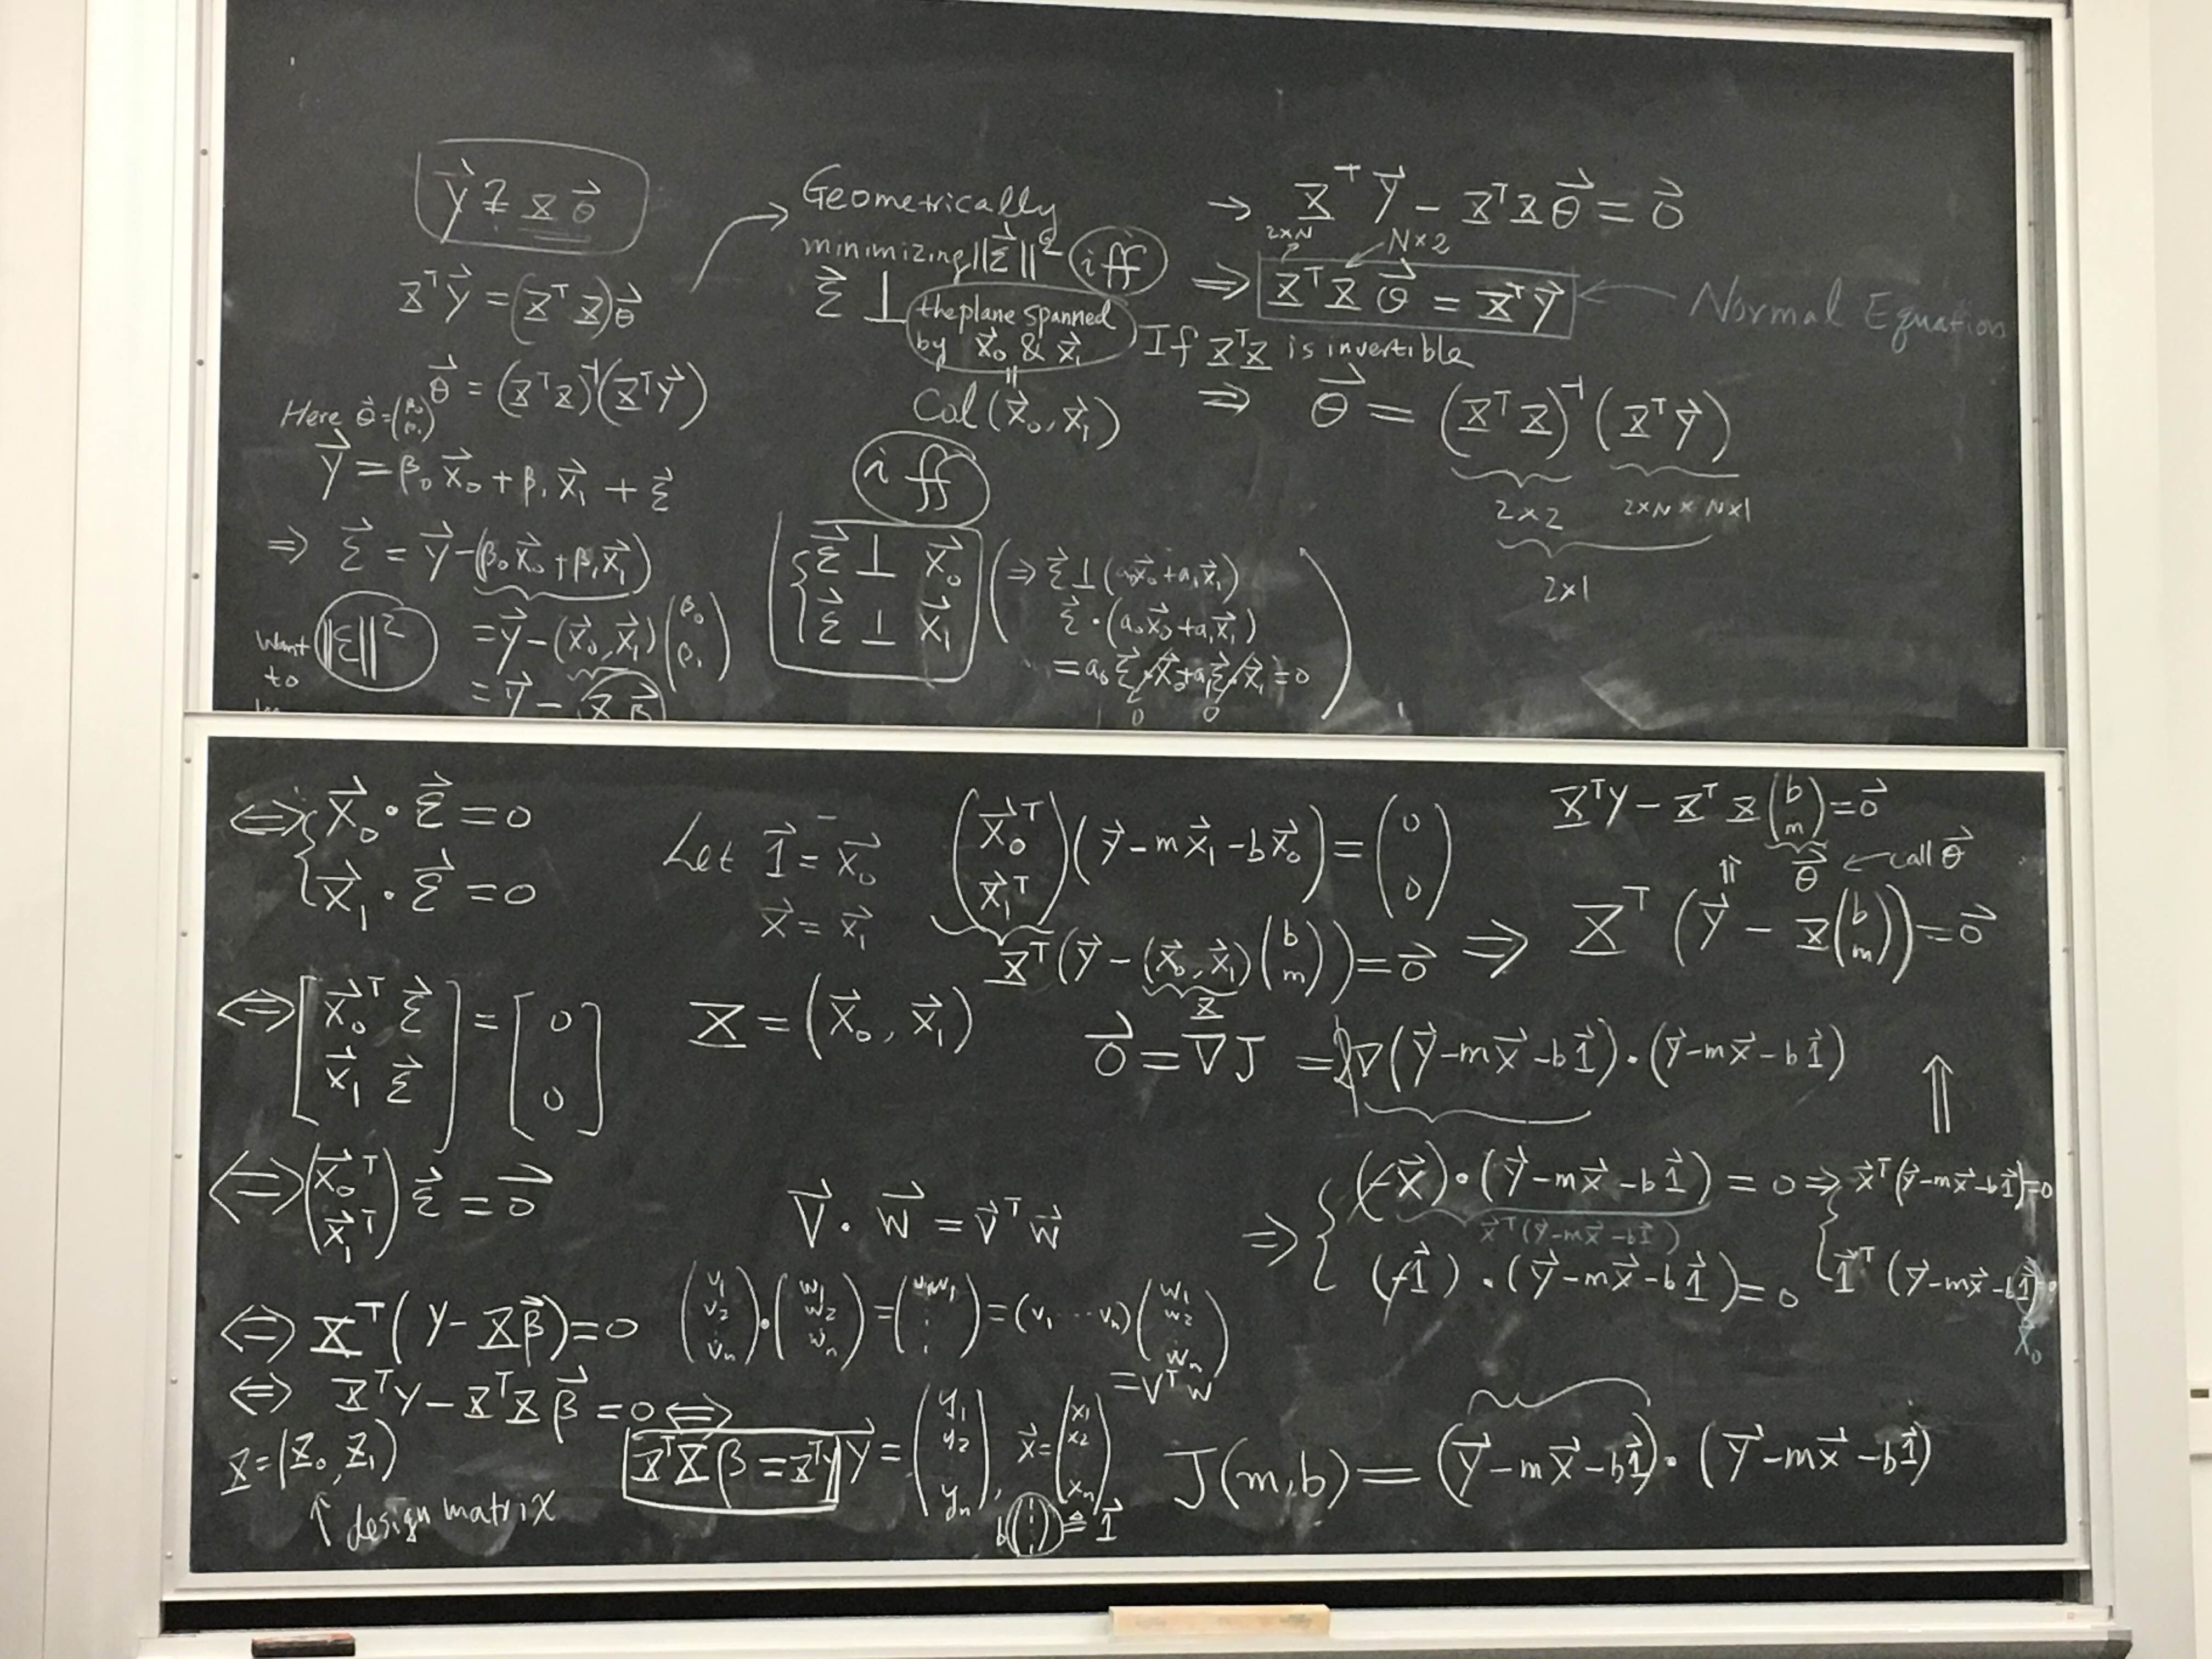
\includegraphics[height=10cm]{LinReg01.JPG}}
\vspace{1pc}
\centerline{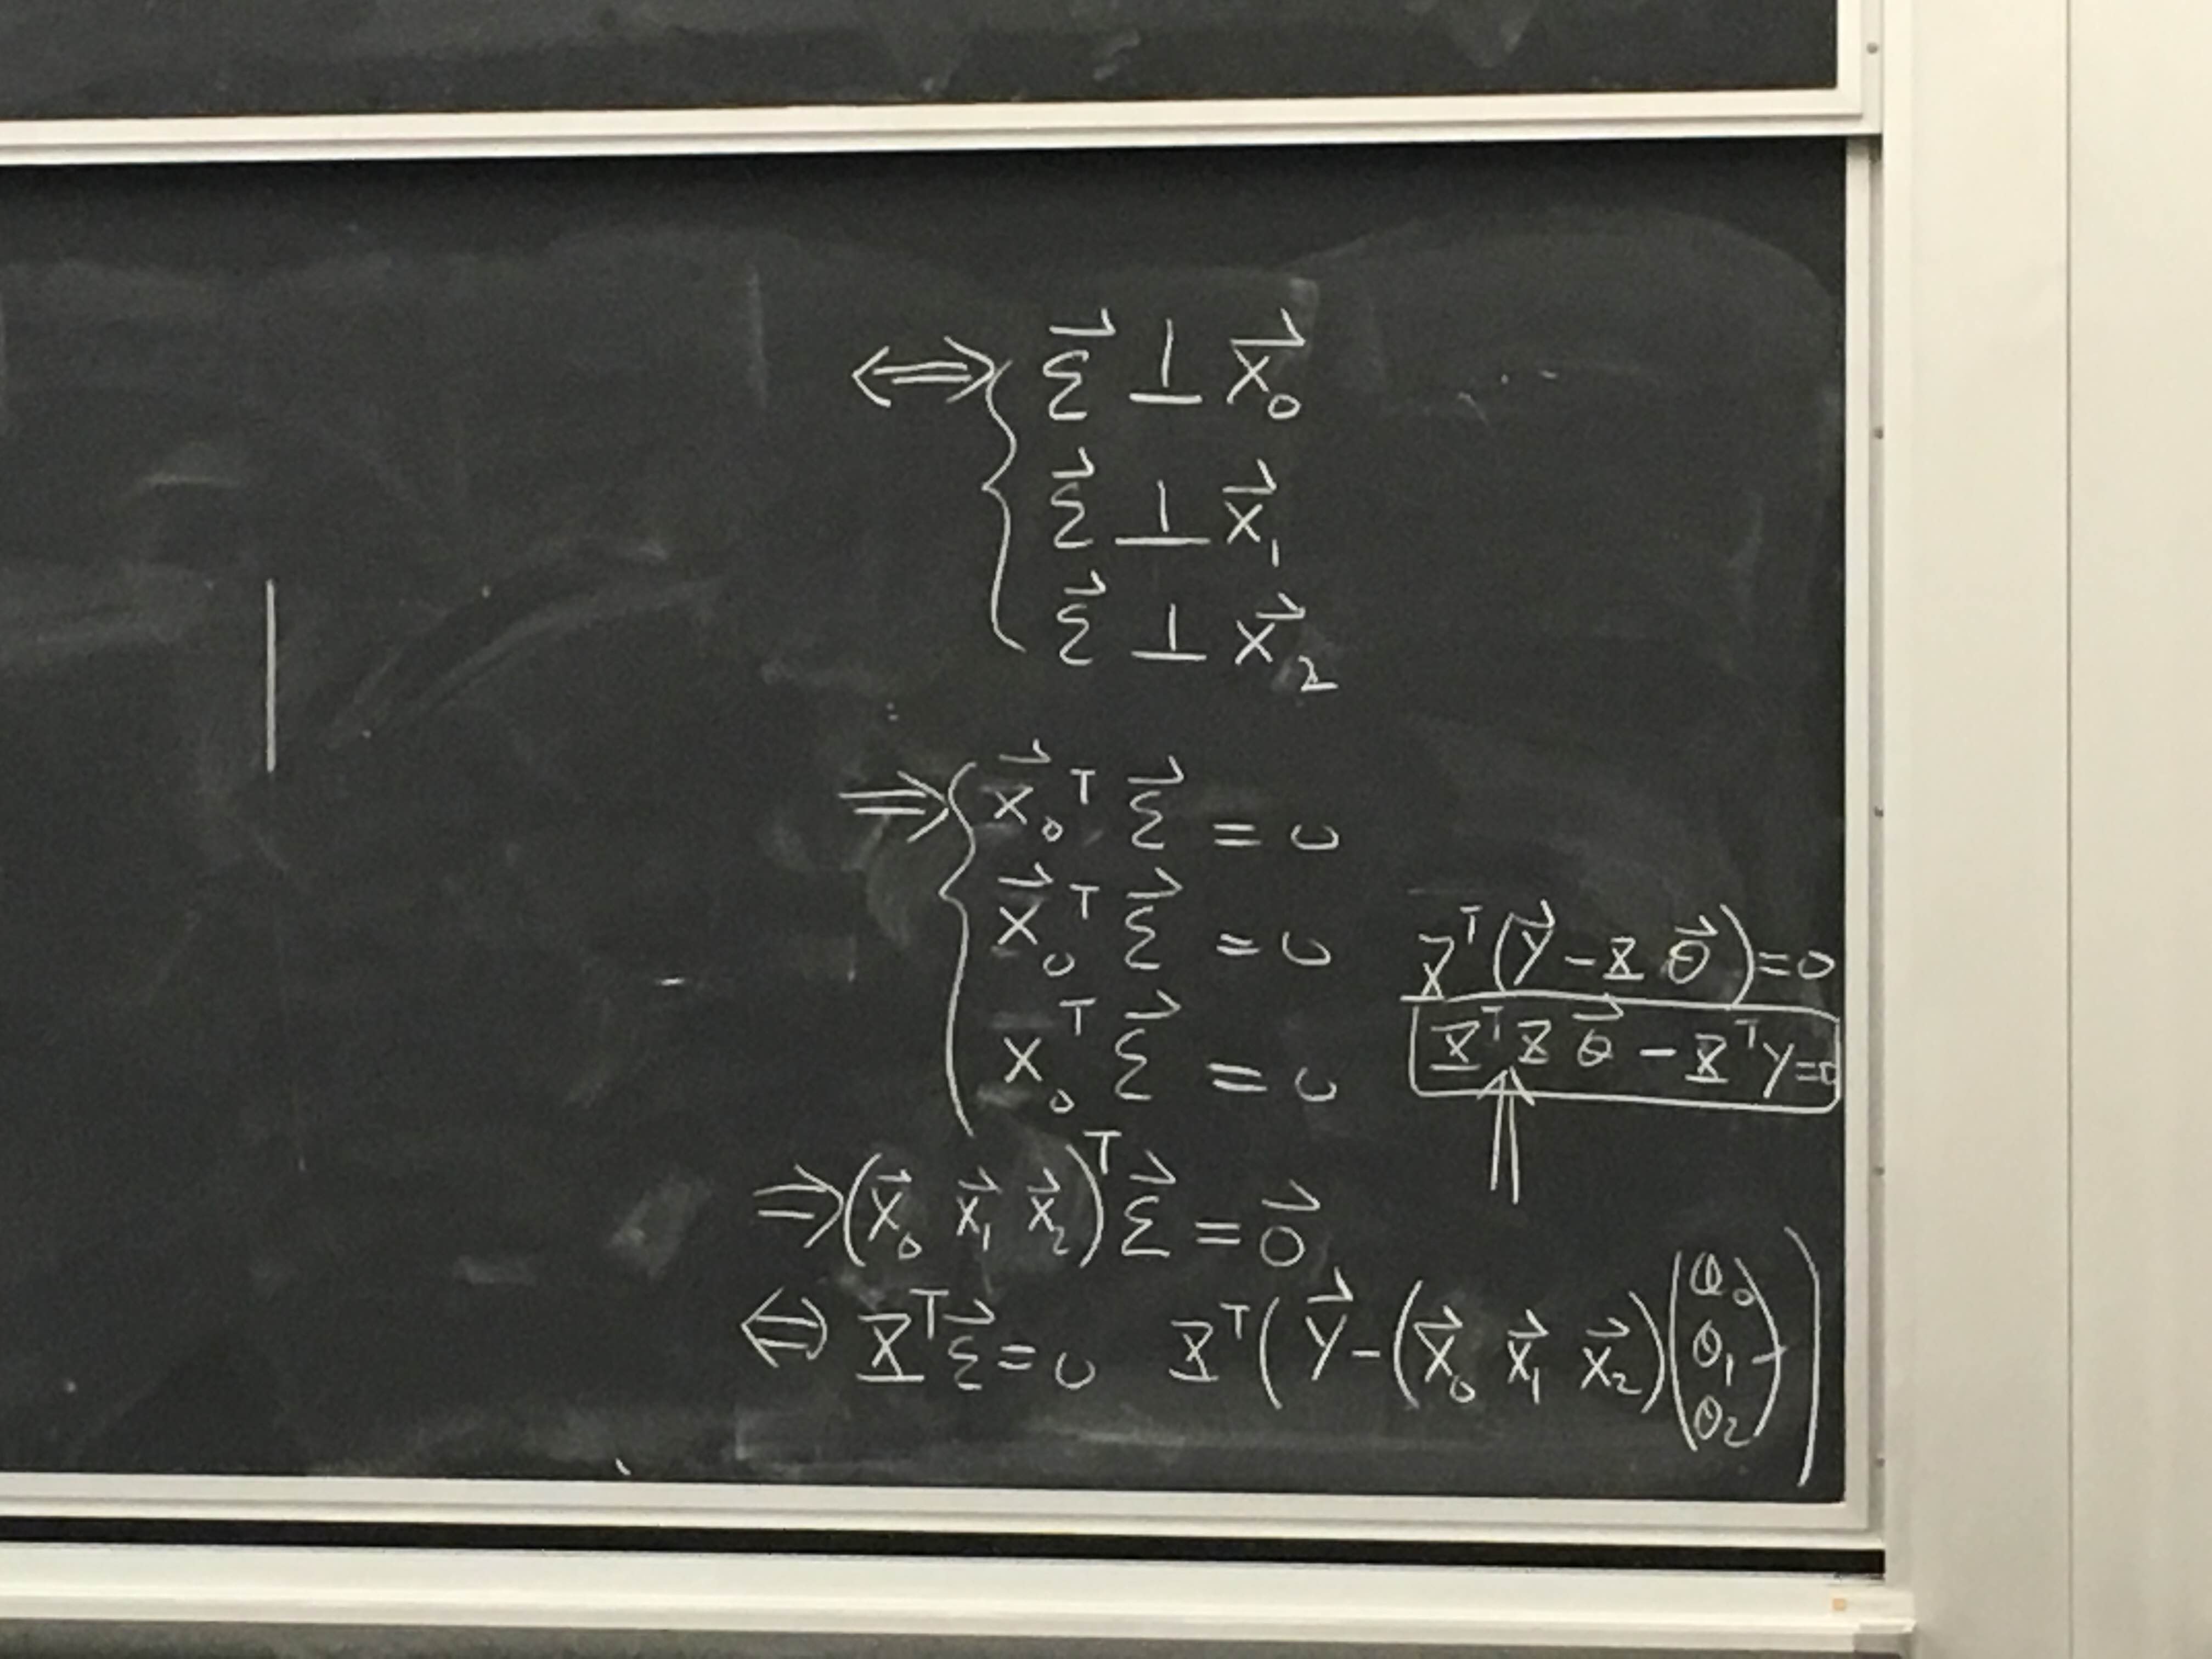
\includegraphics[height=10cm]{LinReg03.JPG}}
\vspace{1pc}

\noindent \textbf{Homework Problem}: Given the four points $(0,1), (2,3), (3,6), (4,8)$.  Find $y= mx + b$ based on Cramer's rule.  Use the normal formula to find the solution and compare it with the first part.  Plot the data points and draw $y=mx + b$.  Find another 100 points near the line $y=mx+b$, then find the least squares approximations again and plot both the data points and the new line.

\vspace{1pc}

\noindent Suppose we want to extend linear regression to multiple dimensions?  For instance, what if instead of fitting points in $\mathbb{R}^2$ with a line, we fit points in $\mathbb{R}^3$ with a plane?  We can generalize what we wrote earlier to parameterize the plane as 

\begin{equation*}
y \;\; =\;\; \theta_0 + \theta_1x_1 + \theta_2 x_2 + \vec{\varepsilon}.
\end{equation*}

\noindent Given a sampling of points $(x_1^{(1)}, x_2^{(1)}, y^{(1)}), \ldots (x_1^{(n)}, x_2^{(n)}, y^{(n)})$ we can then write all of these in matrix form as 

\begin{equation*}
\underbrace{\left [ \begin{array}{c}
y^{(1)} \\
\vdots \\
y^{(n)} \\
\end{array} \right ]}_{\vec{y}} \;\; =\;\; \theta_0 \underbrace{\left [ \begin{array}{c}
1 \\
\vdots \\
1 \\
\end{array} \right ]}_{\vec{x}_0} + \theta_1 \underbrace{\left [ \begin{array}{c}
x_1^{(1)} \\
\vdots \\
x_1^{(n)} \\
\end{array} \right ]}_{\vec{x}_1}   +\theta_2 \underbrace{\left [ \begin{array}{c}
x_2^{(1)} \\
\vdots \\
x_2^{(n)} \\
\end{array} \right ]}_{\vec{x}_2}  + \underbrace{\left [ \begin{array}{c}
\varepsilon^{(1)} \\
\vdots \\
\varepsilon^{(n)} \\
\end{array} \right ]}_{\vec{\varepsilon}}. 
\end{equation*}

\noindent By writing the matrix 

\begin{equation*}
X \;\; =\;\; \left [ \begin{array}{ccc}
\vec{x}_0 & \vec{x}_1 & \vec{x}_2 \\
\end{array} \right ] \hspace{3pc} \vec{\theta} \;\; =\;\; \left [ \begin{array}{c}
\theta_0 \\
\theta_1\\
\theta_2 \\
\end{array} \right ]
\end{equation*}

\noindent we obtain the matrix equation

\begin{equation*}
\vec{y} \;\; =\;\; X \vec{\theta} + \vec{\varepsilon}.
\end{equation*}

\noindent We can solve this again by multiplying this equation by $X^T$ and obtaining a similar equation.  A key difference here is that we would like minimize $||\vec{\varepsilon}||^2$.  How can we do this?

%%%%%%%%%%%%%%%%
\subsection{Geometric/Analytic Approach}

\vspace{1pc}
\centerline{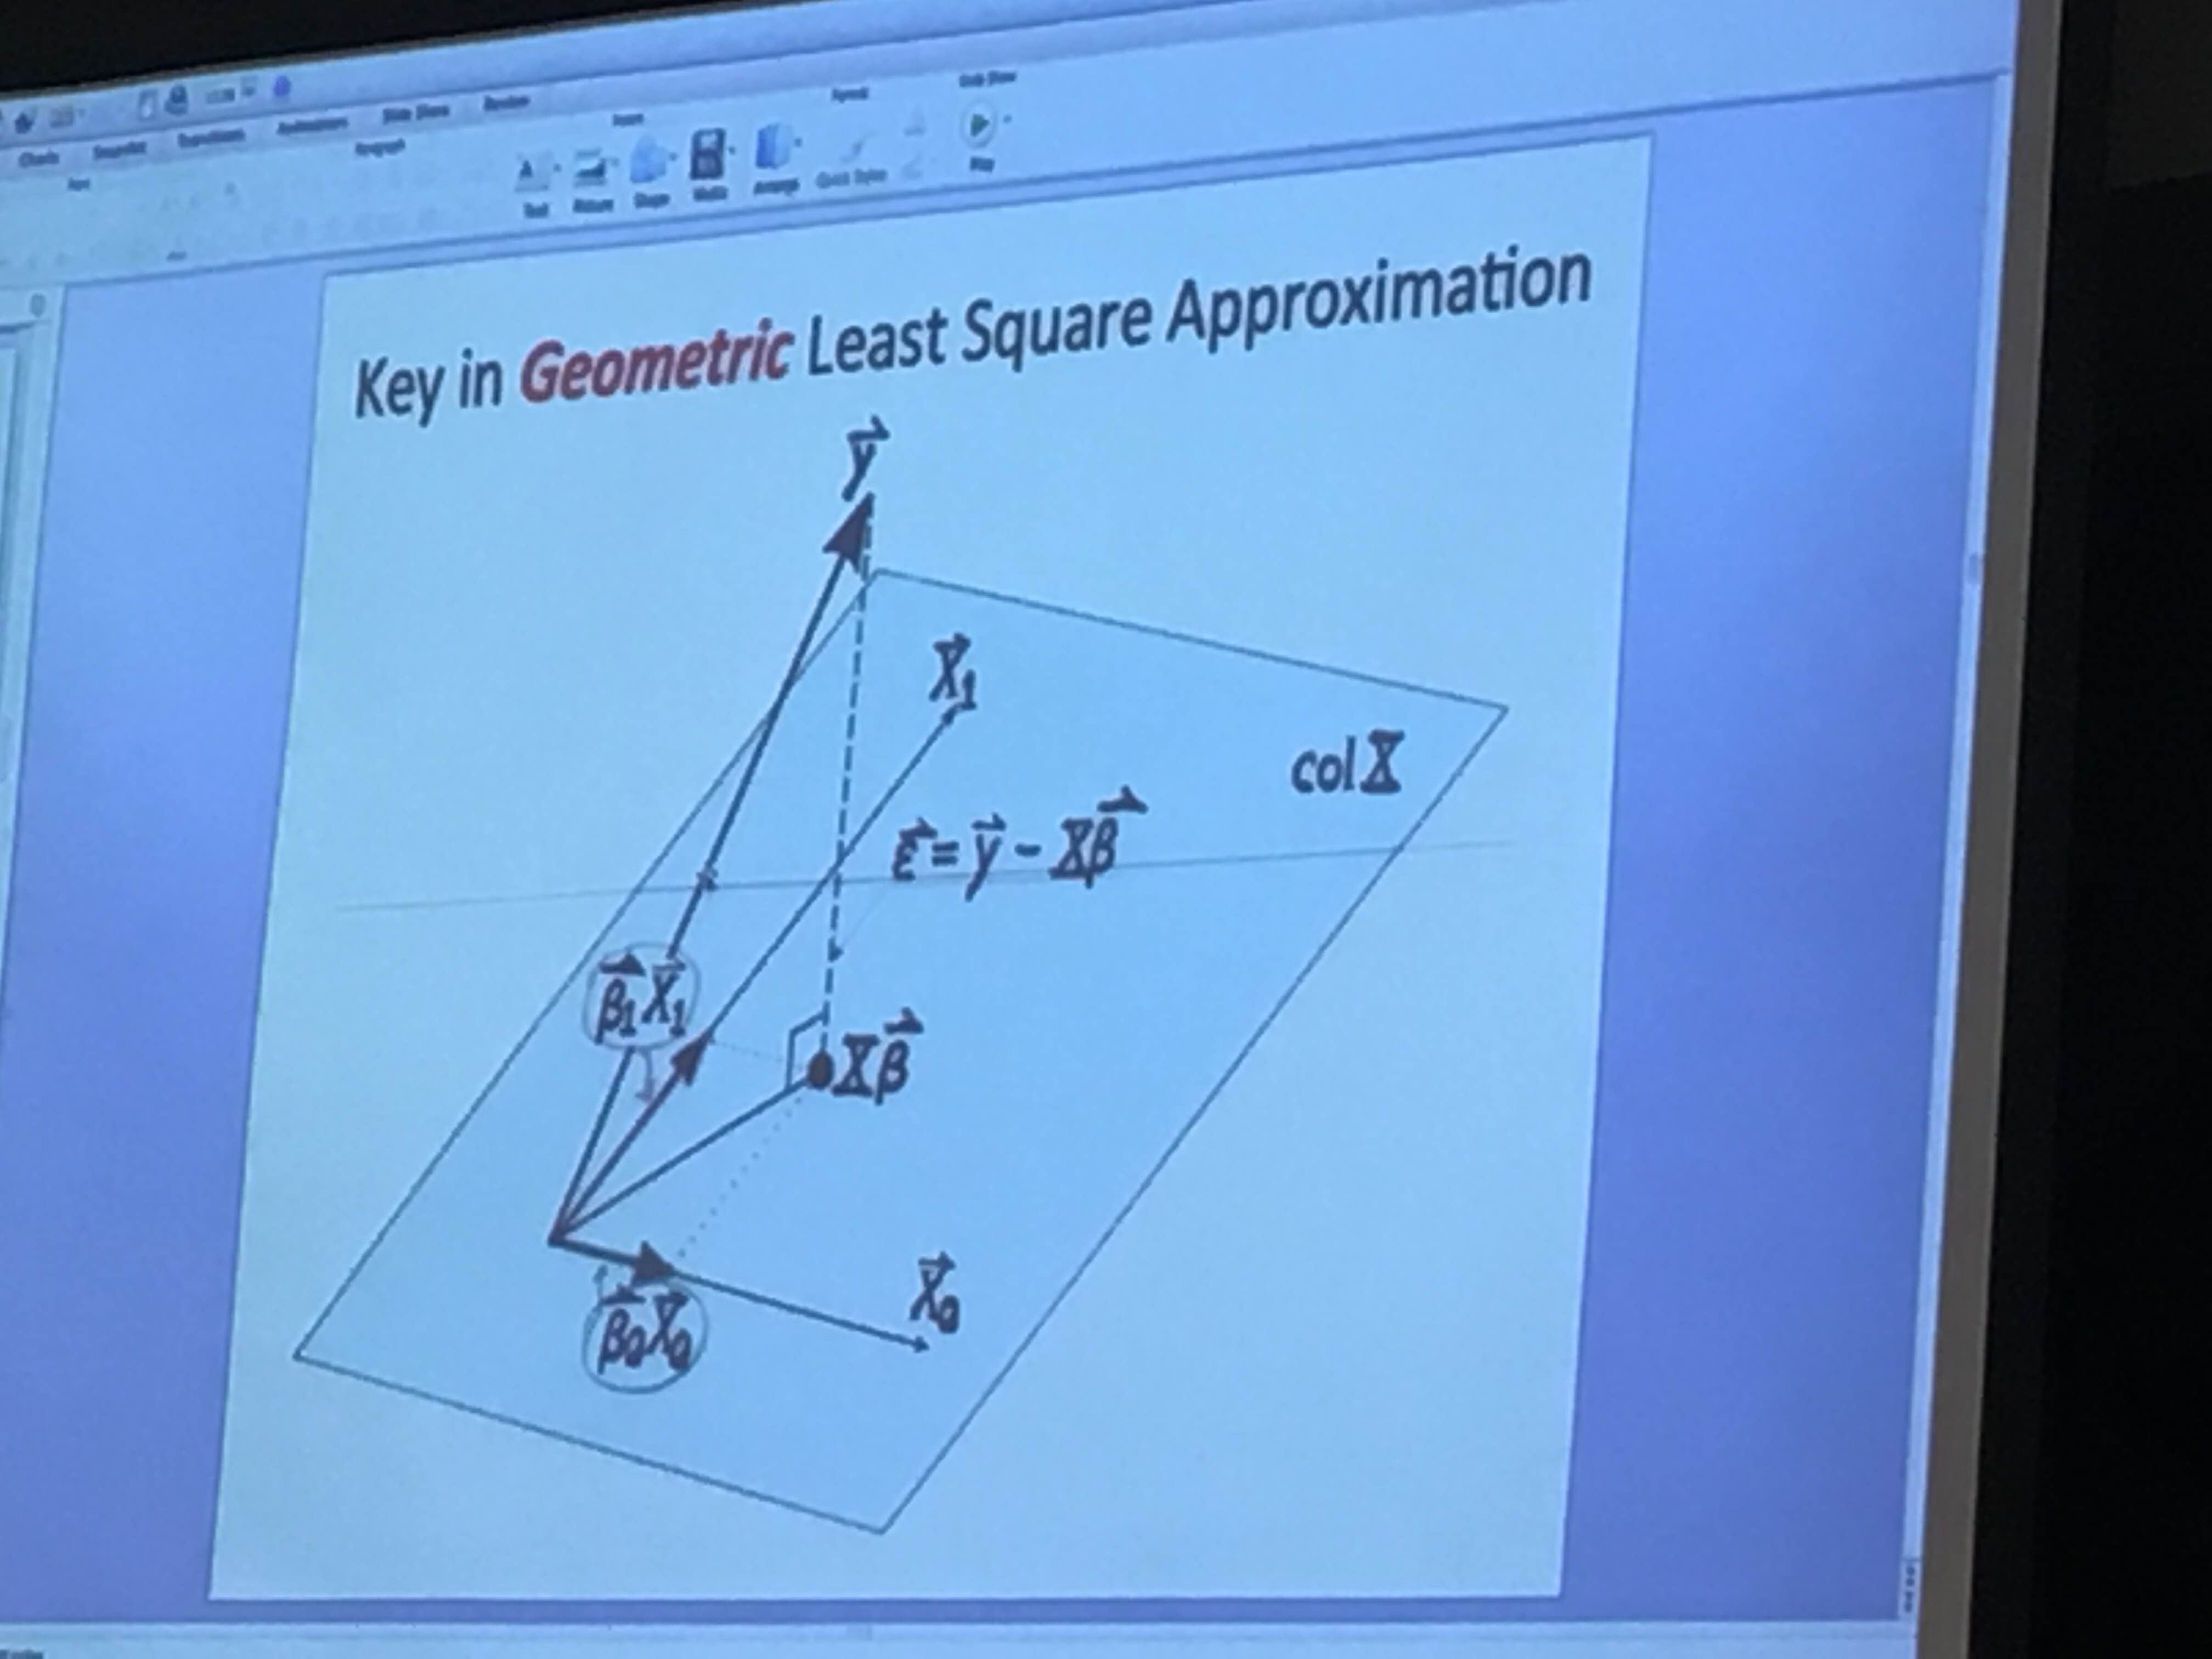
\includegraphics[height=10cm]{GeoKey.JPG}}
\vspace{1pc}

\noindent We can rewrite this equation as $\vec{\varepsilon} = \vec{y} - X \vec{\theta}$, we would like to have an intuitive way of minimizing $\vec{\varepsilon}$.  We can see using an intuitive geometric approach that $\vec{\varepsilon}$ minimizes it's length when it is perpendicular to the column space of $X$.  We can see that $\vec{\varepsilon} \perp \vec{x}_i$ if and only if $\vec{\varepsilon} \cdot \vec{x}_i = \vec{x}_i^T \vec{\varepsilon} = 0$. 

\noindent Observe we can writ these conditions compactly as 

\begin{equation*}
\left [ \begin{array}{c}
\vec{x}_0^T\vec{\varepsilon} \\
\vec{x}_1^T \vec{\varepsilon} \\
\vec{x}_2^T \vec{\varepsilon}\\
\end{array} \right ] \;\; =\;\; \left [ \begin{array}{c}
\vec{x}_0^T \\
\vec{x}_1^T \\
\vec{x}_2^T \\
\end{array} \right ] \left [ \begin{array}{c}
\varepsilon_0 \\
\varepsilon_1 \\
\varepsilon_2 \\
\end{array} \right ] \;\; =\;\; X^T \vec{\varepsilon} \;\; =\;\; 0.
\end{equation*}

\noindent We therefore are able to minimize $||\vec{\varepsilon}||^2$ if and only if $X^T \vec{\varepsilon} = 0$.  Therefore this minimized if and only if $X^T\vec{y} = X^TX \vec{\theta} + X^T \vec{\varepsilon}$ if and only if $X^T \vec{y}= X^TX \vec{\theta}$.  We therefore see that by perturbing our original equation by a noise vector $\vec{\varepsilon}$ our original solution was in fact the optimal solution.  We can conclude that in the case that $X^TX$ is invertible $\vec{\theta} = (X^TX)^{-1} X^T\vec{y}$.  We see here that the main intuition came from a geometric approach to data analysis.

%%%%%%%%%%%%%%
\subsection{Probabilistic Approach -- Maximal Likelihood}

\noindent How can we utilize probability in the case of linear regression?  Observe our original equation again

\begin{equation*}
y^{(i)} \;\; =\;\; \vec{\theta}^T \vec{x}^{(i)} + \varepsilon^{(i)}
\end{equation*}

\noindent where again the $\varepsilon^{(i)}$ is an error term that captures some unmodeled affect or random noise in the system.  We can use probability by making some assumptions on $\varepsilon^{(i)}$.  We can assume that the noise observations $\varepsilon^{(i)}$ are independently and identically distributed (IID) random variables.  It is a good assumption that they are each distributed from a Gaussian distribution with mean $0$ and variance $\sigma^2$.  We can denote this relationship by $\varepsilon^{(i)} \sim N(0, \sigma^2)$.  This is to say explicitly that 

\begin{equation*}
p\left (\varepsilon^{(i)} \right ) \;\; =\;\; \frac{1}{\sqrt{2\pi} \sigma} \exp \left [ - \frac{(y^{(i)} - \theta^T \vec{x}^{(i)})^2}{2\sigma^2} \right ].
\end{equation*}

\noindent By the original equation, we can therefore derive a conditional probability of $\vec{y}^{(i)}$ from the observations $\vec{x}^{(i)}$ and $\vec{\theta}$.  We therefore have that 

\begin{equation*}
p(y^{(i)}|\vec{x}^{(i)}; \vec{\theta}) \;\; =\;\; \frac{1}{\sqrt{2\pi} \sigma} \exp \left [ - \frac{(y^{(i)} - \theta^T \vec{x}^{(i)})^2}{2\sigma^2} \right ]
\end{equation*}

\noindent therefore we can conclude from this that the conditional variable $y^{(i)}|\vec{x}^{(i)}; \vec{\theta} \sim N(\vec{\theta}^T\vec{x}^{(i)}, \sigma^2)$.  These equations however were made for only one observation of $y$.  With observations of this type for $i = 1, \ldots, n$ we are again able to collapse this into a matrix equation

\begin{equation*}
\vec{y} \;\; =\;\; X^T \vec{\theta} + \vec{\varepsilon}.
\end{equation*}

\noindent There are two major interpretations we can make here on the vector $\vec{\theta}$ that we are trying to fit: In one way we can view $\vec{\theta}$ is fixed as a function $\vec{y}$, in another way we can view $\vec{\theta}$ as varying hence $p(\vec{y}|X, \vec{\theta})$ is a function of $\vec{\theta}$.  In this latter case we call it the \textbf{likelihood function}.  We can let 

\begin{equation*}
L(\vec{\theta}) \;\; =\;\; L(\vec{\theta}; X, \vec{y}) \;\; =\;\; p(\vec{y}| \vec{x}; \vec{\theta})
\end{equation*}

\noindent and in the case that the $\varepsilon^{(i)}$ are IID, we then have by the rules of probability that 

\begin{equation*}
L(\vec{\theta}) \;\; =\;\; \prod_{i=1}^n p(y^{(i)} \; | \; \vec{x}^{(i)}; \vec{\theta}) \;\; =\;\; \prod_{i=1}^n \frac{1}{\sqrt{2\pi} \sigma} \exp \left [ - \frac{(y^{(i)} - \theta^T \vec{x}^{(i)})^2}{2\sigma^2} \right ].
\end{equation*}

\vspace{1pc}
\centerline{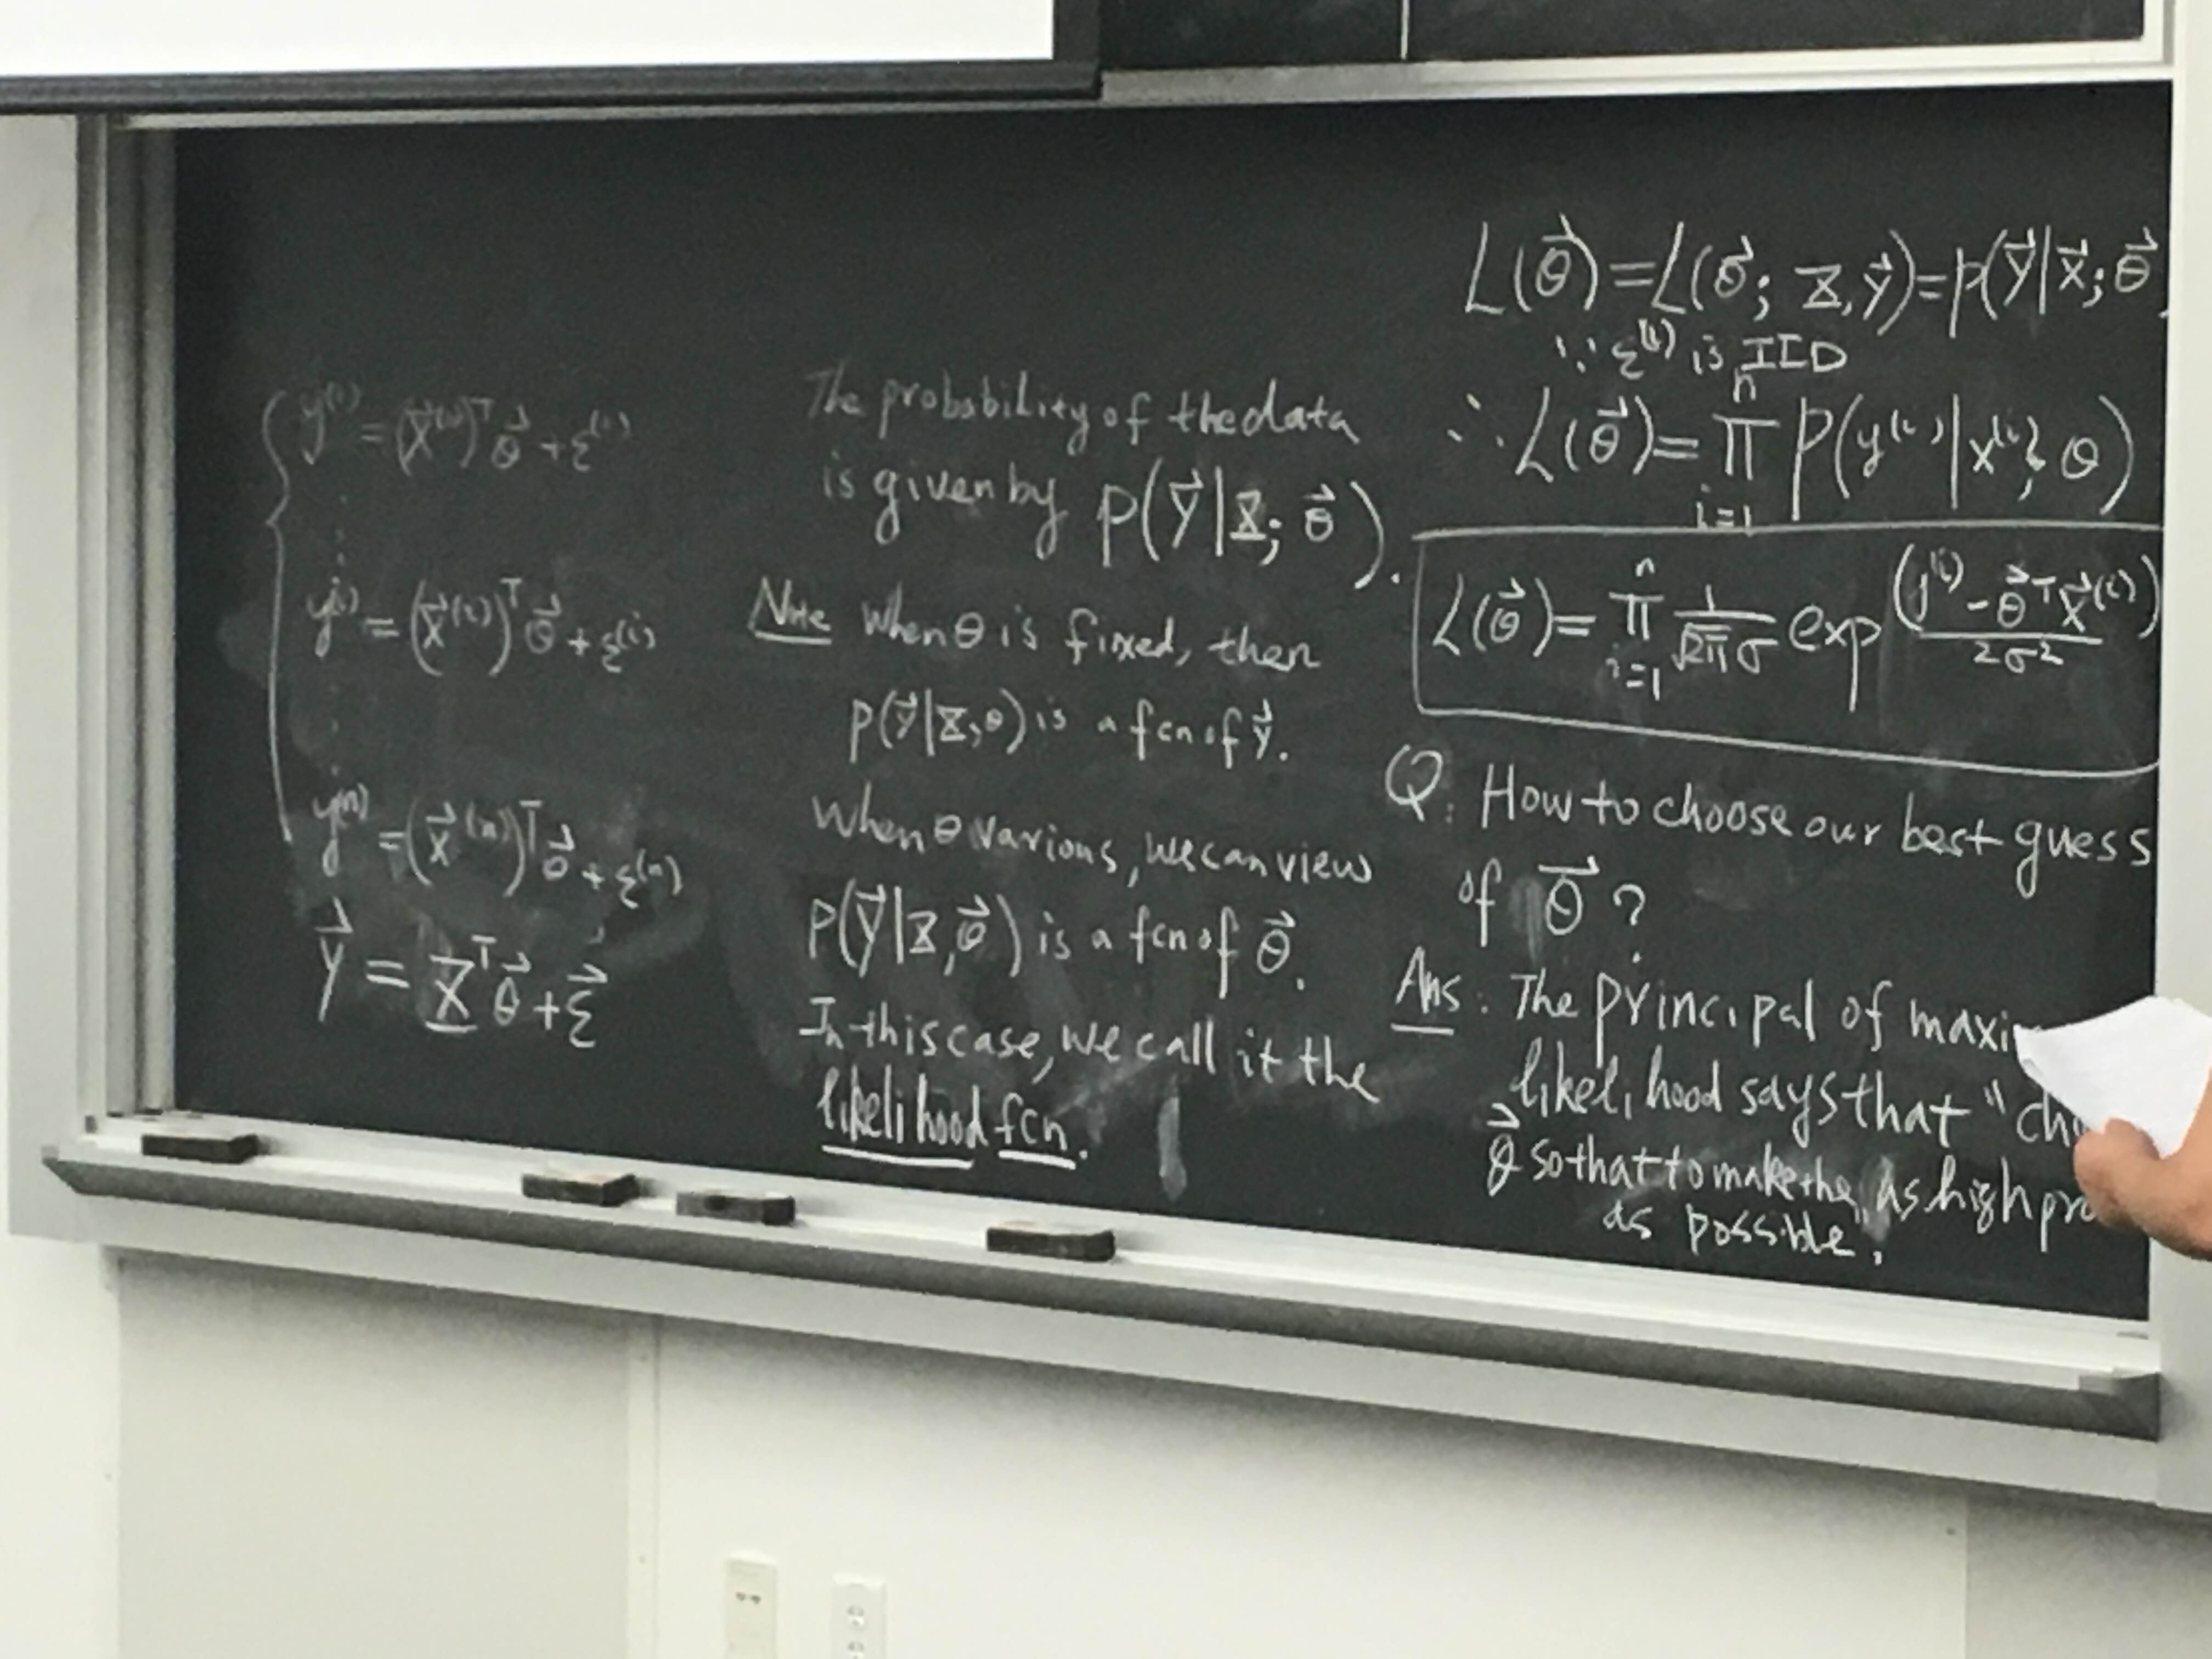
\includegraphics[height=10cm]{LinReg05.JPG}}
\vspace{1pc}

\noindent The question here now becomes how do we choose the optimal $\vec{\theta}$ to get the highest probability as possible?  The \textbf{principle of maximal likelihood} states to choose the $\vec{\theta}$ to give this function the highest probability possible.  In other words, we want to choose $\vec{\theta}$ to maximize $L(\vec{\theta})$.  Analytically this is equivalent to maximizing $\log L(\vec{\theta}) = l(\vec{\theta})$, which from our assumption of IID Gaussian noise, we obtain

\begin{eqnarray*}
l(\vec{\theta}) & = & m \log \frac{1}{\sqrt{2\pi}\sigma} - \frac{1}{2\sigma^2} \sum_{i=1}^n (y^{(i)} - \vec{\theta} \vec{x}^{(i)} )^2.
\end{eqnarray*}

\noindent Note however that in order to maximize $l(\vec{\theta})$ we simply need to minimize the last term in the equation above.  In other words, we want to minimize

\begin{equation*}
\sum_{i=1}^n (y^{(i)} - \vec{\theta} \vec{x}^{(i)})^2 \;\; \equiv \;\; J(\vec{\theta}).
\end{equation*}

\noindent We observe here that we recover our original minimization problem with respect to the function $J(\vec{\theta})$.  







































\end{document}